\documentclass[12pt]{article}
\usepackage[utf8]{inputenc}
\usepackage[T1]{fontenc}
\usepackage{graphicx}
\usepackage{xcolor}

\usepackage{tikz}
\usepackage{calc}
\usepackage{booktabs}
%\usepackage{hyperref}

% colors
\definecolor{color1}{HTML}{000060}
%\definecolor{color1}{HTML}{8C260F}
\definecolor{color2}{HTML}{333333}


% fonts
\usepackage{fontspec}
\defaultfontfeatures{Mapping=tex-text}
\setmainfont
[BoldFont=Lato-Bold.ttf,
ItalicFont=Lato-Italic.ttf,
BoldItalicFont=Lato-BoldItalic.ttf]
{Lato-Regular.ttf}
\newfontfamily\headingfont[ItalicFont=Lato-BlackItalic.ttf]{Lato-Black.ttf}
%%%

\usepackage{geometry}
\geometry{a4paper,
hmargin=20mm,vmargin=20mm,
head=0ex,foot=3ex}

\linespread{1.3}

\usepackage[hang]{caption}
\DeclareCaptionFormat{upper}{#1#2\uppercase{#3}\par}
\captionsetup{labelfont={bf,color=color2},textfont={normalsize,color=color2},format = upper,figurename=FIGURE,tablename=TABLE}

%%% fancy sections
\usepackage{titlesec}
%\titleformat{\chapter}{\headingfont\LARGE\bfseries\scshape\color{color1}}{\thechapter}{1em}{}[\titlerule]
\titleformat{\section}{\color{color1}\headingfont\Large\bfseries\uppercase}{\thesection}{1em}{}[\titlerule]
\titleformat{\subsection}{\color{color1}\headingfont\large\bfseries\uppercase}{\thesubsection}{1em}{}
\titleformat{\subsubsection}{\color{color1}\headingfont\bfseries\uppercase}{\thesubsubsection}{1em}{}
%%%

% head and foot
\usepackage{fancyhdr}
\pagestyle{fancy}
\lhead{}
\chead{}
\makeatletter
\rhead{\color{color2}\@date}
\makeatother
\newlength{\myheight}
\lfoot{
\settoheight{\myheight}{\thepage}
\raisebox{-2ex-0.5\myheight}{
\includegraphics[height=4ex]{logo}}
}
\cfoot{\color{color2}\LaTeX\ template for business reports}
\rfoot{\color{color2}\thepage}
\renewcommand\headrulewidth{0pt}
\renewcommand\footrulewidth{0pt}

%%% picture on cover page
\usepackage{eso-pic}
\newcommand\BackgroundPic{%
\put(0,0){%
\parbox[b][\paperheight]{\paperwidth}{%
\vfill
\centering

\includegraphics[width=\paperwidth,height=\paperheight,%
keepaspectratio]{cover}%
\vfill
}}}
%%%
% custom titlepage
\makeatletter
\renewcommand{\maketitle}{
\thispagestyle{empty}
\AddToShipoutPicture*{\BackgroundPic}
\ClearShipoutPicture
%
\phantom{a}
\vfill
\phantom{a}\hfill
\begin{tabular}[c]{@{}p{0.7\textwidth}@{}}
      \color{white}\headingfont\LARGE\@title\\[1em]
      \color{white}\headingfont\Large\@author\\[2em]
\end{tabular}
%
\clearpage
}
\makeatother
%%%


%%% fancy boxes
\usepackage{tcolorbox}
\usepackage{wrapfig}
\def\fullboxbegin{
\bigskip
\begin{tcolorbox}[colback=color1,colframe=color1,coltext=white,arc=0mm,boxrule=0pt]
}
\def\fullboxend{\end{tcolorbox}\medskip}
%
\def\leftboxbegin{
\begin{wrapfigure}{l}{0.5\textwidth}
\begin{tcolorbox}[colback=color1,colframe=color1,coltext=white,arc=0mm,boxrule=0pt]
}
\def\leftboxend{
\end{tcolorbox}
\end{wrapfigure}
}
%
\def\rightboxbegin{
\begin{wrapfigure}{r}{0.5\textwidth}
\begin{tcolorbox}[colback=color1,colframe=color1,coltext=white,arc=0mm,boxrule=0pt]
}
\def\rightboxend{
\end{tcolorbox}
\end{wrapfigure}
}
%
\newcounter{frames}
\def\frameboxbegin#1{
\bigskip
\refstepcounter{frames}
\begin{tcolorbox}[colback=white,colframe=color1,arc=0mm,title={\MakeUppercase{\textbf{Frame \arabic{frames}}: #1}}]
}
\def\frameboxend{
\end{tcolorbox}
}
%%%

\usepackage{lipsum}

%%%%%%%%%%%%%%%
% Title Page
\title{Robotic activities in Technovision \newline \normalsize{Early Mastery - Playful Coding}}
\author{\small{Laboratoire Electronique, Informatique, Image \newline Universit\'e de Bourgogne - Le Creusot - France}}
\date{\today}
%%%%%%%%%%%%%%%

\begin{document}
\maketitle

\tableofcontents
\clearpage

\section{Activity \# 1 - First Steps}
\clearpage
\section{Activity \# 2 - Like in Ski}


\frameboxbegin{Summary of the Activity}
Total duration: 30 minutes
The required equipment for this activities should be:
\begin{itemize}
\item 1 robot POB;
\item 1 computer with Risbee software installed;
\item 1 mini-USB cable;
\item 2 objects/targets
\item the booklet ``Quick Start Risbee''.
\end{itemize}
\frameboxend

\frameboxbegin{Motion - 5 minutes}
\begin{description}
\item[Objective:] To be able to move forward the robot.
\item[I am learning:] \hfill \\ \vspace{-4ex}
  \begin{itemize}
  \item To order the icons in order to make a simple program;
  \item To move the robot forward;
  \item The concept of trajectory.
  \end{itemize}
\end{description}
\frameboxend

\frameboxbegin{Slalom - 20 minutes}
\begin{flushleft}
\begin{description}
\item[Objectives:] To move the robot from a landmark ``A'' to a landmark ``C'' passing by a landmark ``B'' by bending as depicted in Fig.\,\ref{fig:s}. The player can chose either to stop at each landmark after each bend or to travel in one shot.
\begin{minipage}[c]{\textwidth}
\centering
\tikzstyle{target}=[circle,thick,minimum size=2cm,draw=blue!80,fill=blue!20]
\vspace{1ex}
\begin{tikzpicture}[>=latex,text height=1ex,text depth=0.25ex]
  \matrix[row sep=1cm,column sep=1.5cm] {
    \node (A) [target] {A}; &
    &
    \node (B) [target] {B}; &
    &
    \node (C) [target] {C}; &
    \\
  };
  \path[->]
  (A) edge[bend left=90,thick] (B)
  (B) edge[bend right=90,thick] (C);
\end{tikzpicture}
\captionof{figure}{Landmarks positioning.}\label{fig:s}
\end{minipage}
\item[I am learning:] \hfill \\ \vspace{-1ex}
  \begin{itemize}
  \item To discover some additional icons;
  \item To move the robot until a given landmark;
  \item The concept of trajectory;
  \item The concept of angle;
  \item The change of direction.
  \end{itemize}
\end{description}
\end{flushleft}
\frameboxend

\frameboxbegin{Race - 5 minutes}
\begin{flushleft}
\begin{description}
\item[Objective:] To make a race between two robots. Move the position of the landmark ``B'' and ``C'' which will have to be reached by the players.
\item[I am learning:] \hfill \\ \vspace{-1ex}
  \begin{itemize}
  \item To discover some additional icons;
  \item To control the speed of the engines;
  \item To challenge other players.
  \end{itemize}
\end{description}
\end{flushleft}
\frameboxend

\clearpage
\section{Activity \# 3 - The Musical Chair}
\clearpage

% \section{Features commands}

% \subsection{Pictures used}

% \noindent
% Cover picture filename (in titlepage): \texttt{cover}\\
% Logo filename (in foot): \texttt{logo}

% \subsection{Boxes}

% \begin{verbatim}
% \fullboxbegin
% Content
% \fullboxend
% \end{verbatim}

% \begin{verbatim}
% \leftboxbegin
% Content
% \leftboxend
% \end{verbatim}

% \begin{verbatim}
% \rightboxbegin
% Content
% \rightboxend
% \end{verbatim}

% \begin{verbatim}
% \frameboxbegin{Frame Title}
% Content
% \frameboxend
% \end{verbatim}

% \newpage

% \section{First section}
% \lipsum[1]

% \fullboxbegin
% \lipsum[1]
% \fullboxend

% \lipsum[1]

% \subsection{First subsection}
% \lipsum[1]

% \leftboxbegin
% Lorem ipsum dolor sit amet, consectetuer adipiscing elit. Ut purus elit, vestibulum ut, placerat ac, adipiscing vitae, felis. Curabitur dictum gravida mauris. Nam arcu libero, nonummy eget, consectetuer id, vulputate a, magna. Donec vehicula augue eu neque. 
% \leftboxend

% \lipsum[1-2]

% \rightboxbegin
% \begin{itemize}
%  \item Lorem ipsum
%  \item Lorem ipsum
% \end{itemize}
% \rightboxend

% \lipsum[1]

% \subsubsection{First subsubsection}

% \lipsum[1]

% \begin{figure}[!h]
% \centering
% 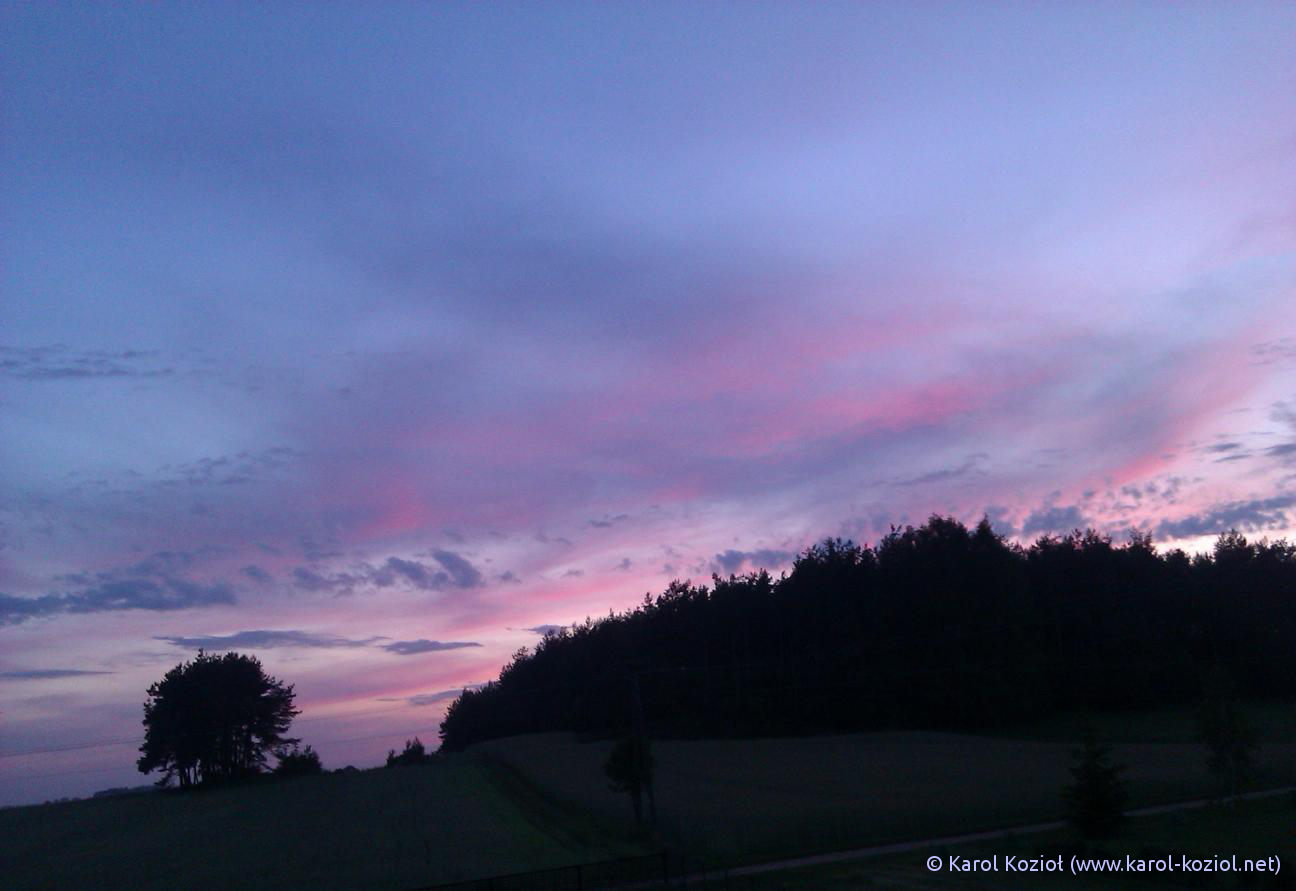
\includegraphics[width=0.5\textwidth]{sky.jpg}
% \caption{The sky is the limit.}
% \end{figure}

% \section*{Unnumbered section}
% \lipsum[1]

% \begin{figure}[!h]
% \centering
% 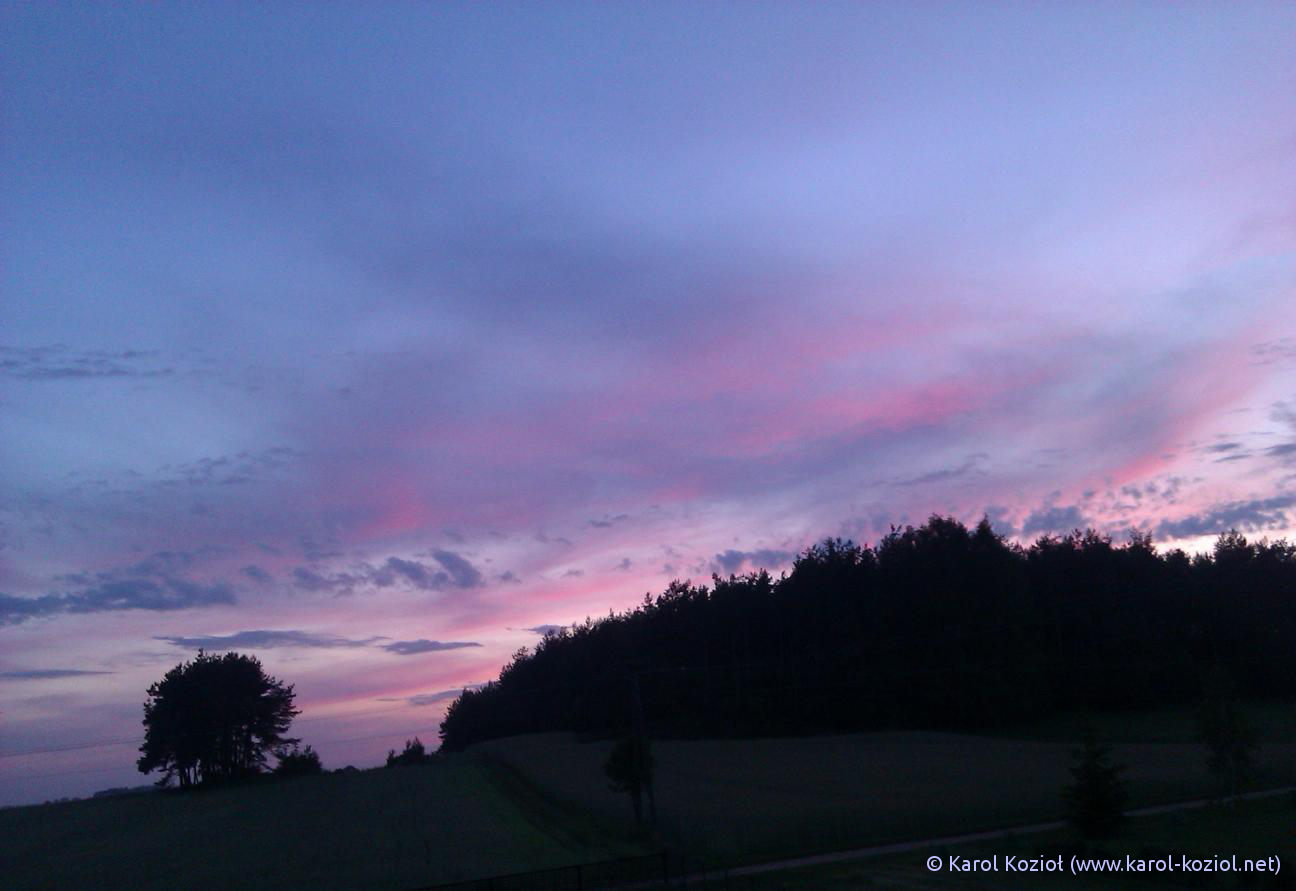
\includegraphics[width=0.5\textwidth]{sky.jpg}
% \caption*{The sky is the limit.}
% \end{figure}

% \section{Second section}

% \lipsum[1]
% \begin{table}[!h]
% \centering
% \caption{Sample table.}
% \begin{tabular}{cccc}
% \toprule
% Value 1 & Value 2 & Value 3 & Value 4\\
% \midrule
%  odd     & odd   & odd & 1.00 \\
%  even    & even  & even& 1.00 \\
%  odd     & odd   & odd & 1.00 \\
%  even    & even  & even& 1.00 \\
% \bottomrule
% \end{tabular}
% \end{table}

% \lipsum[1]

% \frameboxbegin{Sample frame}
% \lipsum[1]
% \frameboxend

\end{document}          
